%%%%%%%%%%%%%%%%%%%%%%%%%%%%%%%%%%%%%%%%%
% FRI Data Science_report LaTeX Template
% Version 1.0 (28/1/2020)
%
% Jure Demšar (jure.demsar@fri.uni-lj.si)
%
% Based on MicromouseSymp article template by:
% Mathias Legrand (legrand.mathias@gmail.com)
% With extensive modifications by:
% Antonio Valente (antonio.luis.valente@gmail.com)
%
% License:
% CC BY-NC-SA 3.0 (http://creativecommons.org/licenses/by-nc-sa/3.0/)
%
%%%%%%%%%%%%%%%%%%%%%%%%%%%%%%%%%%%%%%%%%

%----------------------------------------------------------------------------------------
%	PACKAGES AND OTHER DOCUMENT CONFIGURATIONS
%----------------------------------------------------------------------------------------
\documentclass[fleqn,moreauthors,10pt]{ds_report}
\usepackage[slovene]{babel}
\usepackage{hyperref}
\usepackage{enumitem}
\usepackage[T1]{fontenc}
\usepackage[utf8]{inputenc}
\usepackage{float}
\usepackage{fancyvrb}
\graphicspath{{fig/}}
\usepackage{listings}
\usepackage{fvextra}

\lstset{
    extendedchars=true,
    inputencoding=utf8,
    literate={č}{{\v{c}}}1 {ž}{{\v{z}}}1 {š}{{\v{s}}}1
             {Č}{{\v{C}}}1 {Ž}{{\v{Z}}}1 {Š}{{\v{S}}}1
}
%----------------------------------------------------------------------------------------
%	ARTICLE INFORMATION
%----------------------------------------------------------------------------------------

% Header
\JournalInfo{FRI Natural language processing course 2026}

% Interim or final report
\Archive{Project report}
%\Archive{Final report}

% Article title
\PaperTitle{
FRI ReferatBot – Domain-Specific assistant for UL FRI Student Affairs Office
}

% Authors (student competitors) and their info
\Authors{Gašper Kolbezen, Samo Hribar and Gašper Suhadolnik}

% Advisors
\affiliation{\textit{Advisors: Slavko Žitnik}}

% Keywords
\Keywords{Retrieval-Augmented Generation, Large Language Models, Domain-Specific Chatbot, Student Affairs, Slovenian NLP}
\newcommand{\keywordname}{Keywords}


%----------------------------------------------------------------------------------------
%	ABSTRACT
%----------------------------------------------------------------------------------------

\Abstract{
General-purpose Large Language Models (LLMs) are highly capable at open-domain conversation,
but they frequently hallucinate when asked institution-specific questions they were not trained on.
This project addresses that limitation by building \textbf{ReferatBot}, a domain-specific conversational assistant
for the Student Affairs Office (Referat) of the Faculty of Computer and Information Science
at the University of Ljubljana (UL FRI).
The assistant serves the faculty's enrolled students by answering questions about enrolment procedures,
exam regulations, thesis submission, student status, fees, and related administrative topics.
We implemented a Retrieval-Augmented Generation (RAG) pipeline grounded in a curated corpus of
427 scraped web pages and 33 official PDF rulebooks, totalling approximately 500,000 words.
This report covers the project motivation, a survey of related work, the implemented methodology,
and an evaluation of the system.
}

%----------------------------------------------------------------------------------------

\begin{document}

% Makes all text pages the same height
\flushbottom

% Print the title and abstract box
\maketitle

% Removes page numbering from the first page
\thispagestyle{empty}

%----------------------------------------------------------------------------------------
%	ARTICLE CONTENTS
%----------------------------------------------------------------------------------------

\section*{Introduction}
Students at university faculties routinely encounter administrative questions,
which are answered on the UL FRI website and in official study regulations,
yet students frequently contact the Student Affairs Office (Referat) by email or in person
for answers that are already publicly accessible.
This imposes a significant workload on administrative staff and introduces delays for students.

General-purpose LLMs such as GPT or Llama cannot always reliably answer these questions:
Some UL FRI-specific rules (e.g., the precise ECTS thresholds for year advancement) or even FRI specific questions
are hard for LLMs to answer correctly and the models hallucinate plausible-sounding but incorrect answers.
The goal of this project was to close that gap by building a specialised assistant
that retrieves factual information from a verified, institution-specific knowledge base
before generating a response.

Our target domain was the UL FRI Student Affairs Office.
The closest existing analogue within the University of Ljubljana is the AI student assistant
deployed on the Faculty of Mechanical Engineering (UL FS) website,
which is embedded as a live chat widget under the title ``AI pomoč za študente UL FS''.
Our system aims to replicate and extend this concept for UL FRI,
with reproducible code and open dataset.

%gasperk
% To create our dataset, we gathered data by scraping the UL FRI website and collecting UL rulebooks and administrative PDFs, which are accessible online.
% We then converted this data into Markdown for LLM parsing. To create an evaluation corpus, we wrote 31 questions and evaluated our system on them.

% The core implementation includes a Retrieval-Augmented Generation (RAG) \cite{lewis2020retrieval} architecture. We used the Slovenian GaMS model to process user intents and generate answers.
% For the retrieval pipeline, we chunked our parsed Markdown documents, generated vector embeddings using a BGE-m3 based model \cite{baai3}, and stored them in PostgreSQL using the pgvector extension.

System prompting enforces a ``Student Affairs Advisor'' persona with guardrails against out-of-domain questions and instructions to direct unanswerable queries to the Referat office.
The system is evaluated by comparing three embedding models on a handcrafted FAQ dataset.

%gaspers
\section*{Related Work}
\subsection*{Domain-Specific Knowledge Incorporation}
Incorporating domain-specific knowledge into LLMs is done through the following main approaches: prompt engineering, retrieval-augmented generation (RAG) \cite{lewis2020retrieval}, and fine-tuning.
Prompt engineering is the fastest and cheapest method, where carefully designed prompts provide the model with additional knowledge at runtime. While this technique is fast and quick to set up, it offers limited depth and accuracy in some cases, including domain tasks.

RAG \cite{lewis2020retrieval} solves this issue by connecting the model to external knowledge sources, improving accuracy and transparency, though at the cost of added system complexity and latency. Knowledge is obtained from internal documents, websites, PDFs, company databases etc. and is typically stored in some vector database, such as FAISS, Pinecone, Weaviate, etc. During inference, relevant documents are first retrieved from the database based on user prompt using vector search, and are then passed on to the underlying LLM, which generates the answer.

Fine-tuning embeds domain expertise directly into the model, delivering high performance and consistency for specialized tasks, but requires significant data, time, and ongoing maintenance. It is also harder to update or add new knowledge, which is done by additional fine-tuning of the model.

In practice, these methods are often combined, with RAG \cite{lewis2020retrieval} providing dynamic knowledge, fine-tuning ensuring consistent behavior, and prompting orchestrating interactions.

\subsection*{Existing Solutions}
There are many existing university chatbot solutions using RAG architecture that differ in used technologies and purpose.
One example of such a system is a chatbot developed for Mississippi State University by Neupane et al., which uses BarkPlug v2 \cite{neupane2024questions} architecture. For context retrieval it uses an embedding model for vectorization of external data sources and Chroma DB vector database. Actual context retrieval is done by a retriever technique provided by LangChain \cite{langChain} using Maximum Marginal Relevancy and Similarity Search methods. For the underlying LLM, it utilizes OpenAi's gpt-3.5-turbo. The system achieved a mean RAGAS score of 0.96, and has proven itself to be practical and effective for real-world usage through various qualitative experiments.

Other examples of such chatbots are Meri AI \cite{meriAi} and AceIt-ECE-Capstone \cite{aceIt}. Meri AI \cite{meriAi} is a campus intelligence system, which runs a LangGraph workflow \cite{langChain} for intent classification, route detection, context retrieval, and response generation. It uses Supabase PostgreSQL with pgvector as knowledge database containing content scraped from university resources.
AceIt-ECE-Capstone \cite{aceIt} is a course assistant focused on study help. It uses RAG \cite{lewis2020retrieval} pipeline where course data is embedded with Amazon Titan Text Embeddings v2 and stored in Amazon RDS PostgreSQL. It uses Llama 3.3 to generate responses based on user query and retrieved database knowledge.

Another example of a university chatbot is a virtual AI assistant developed by the Faculty of Mechanical Engineering (Fakulteta za strojništvo) at the University of Ljubljana. Unfortunately, it seems that there is no publicly available information about its architecture and even when asked the bot itself, it was unable to answer it accurately. It was, however, able to explain that the data used to provide user query with relevant context comes from UL FS webpage and standard Q\&A entries.


%------------------------------------------------

\section*{Methods}

\subsection*{Dataset}
For the purpose of this project, we first curated a dataset. This was done by scraping 427 HTML pages from UL FRI websites and collecting 33 official PDF rulebooks.
Using Microsoft's MarkItDown, we converted these into Markdown. Next, we performed data sanitization by removing HTML navigation menus, stripping standalone hyperlinks, resolving PDF layout artifacts (e.g., mid-sentence line breaks), and collapsing whitespace.
The final, cleaned corpus contains approximately 500,000 words of relevant administrative text.

\subsection*{Vector storage and retrieval}
For vector storage and retrieval, we utilize TimescaleDB with the pgvector extension, managed through the \texttt{timescale-\allowbreak vector} Python client.
Document chunks are represented as 1024-dimensional vectors generated by the BAAI/bge-m3\cite{baai3} model, which was selected for its strong performance in multilingual tasks.
To ensure efficient and scalable retrieval, we implemented a Hierarchical Navigable Small World (HNSW)\cite{hmsw} index using cosine similarity.
The database schema stores the raw text content alongside JSONB metadata (including source file origin, chunk identifiers, and document headers) and UUIDs generated from timestamps.
This architecture supports both semantic similarity search and precise metadata filtering, such as time-range queries or source-specific retrieval.


\subsection*{Large Language Model}
The synthesis component of our RAG system is powered by the GaMS-9B-Instruct-Nemotron model, a 9-billion parameter instruct-tuned model optimized for the Slovenian language.
The model is deployed locally using the Hugging Face \texttt{pipeline} API on NVIDIA hardware (\texttt{cuda}).
Since the Gemma~2 chat template does not natively support a \texttt{system} role, system instructions are instead injected as the opening user turn, with the model acknowledging them in a synthetic assistant turn before the actual query is posed.
This three-turn pattern reliably activates instruction-following behaviour without modifying the model weights.
We employ a structured prompting strategy where the model is provided with a comprehensive system prompt that defines its role as a specialized Student Affairs Advisor for UL FRI.
This prompt enforces strict operational constraints: the assistant must use the provided context exclusively, remain transparent when information is missing, maintain a professional tone, and strictly adhere to security guidelines (such as refusing to reveal internal instructions).
During inference, the top-k relevant chunks retrieved from the vector store are formatted into a JSON structure and passed to the model alongside the user's query to ensure the generated responses are grounded in the verified faculty knowledge base.
Listing~\ref{lis:sysprompt} shows an excerpt of the system prompt.

\begin{lstlisting}[frame=single, breaklines=true, caption={Excerpt of the system prompt.}, label={lis:sysprompt}]
# Role and Purpose
You are an AI assistant for the study process at FRI.
Your task is to formulate a meaningful response
based on the question asked and the context from
the knowledge base.

# Guidelines:
1. Respond in the user's language.
2. Use only information from
   the provided context.
4. Be transparent when there is not enough
   information for a complete answer.
9. If the question is not related to studies:
    "I cannot help you with matters that are not related to
    studies at FRI."
\end{lstlisting}


\subsection*{System Architecture}

Figure~\ref{fig:architecture} shows the full deployment architecture.
The online path (left to right) covers query handling: the user's message travels from the browser frontend to the FastAPI backend, which embeds the query, retrieves the top-$k$ chunks from TimescaleDB/pgvector, and passes them together with the query to the Synthesizer. The Synthesizer constructs the three-turn message list and calls GaMS-9B-Instruct-Nemotron, whose answer is returned to the user. The offline ingestion path (top) shows how the corpus of HTML pages and PDFs is processed by MarkItDown and the chunker before embeddings are written to the vector store.

\begin{figure*}[htbp]\centering
    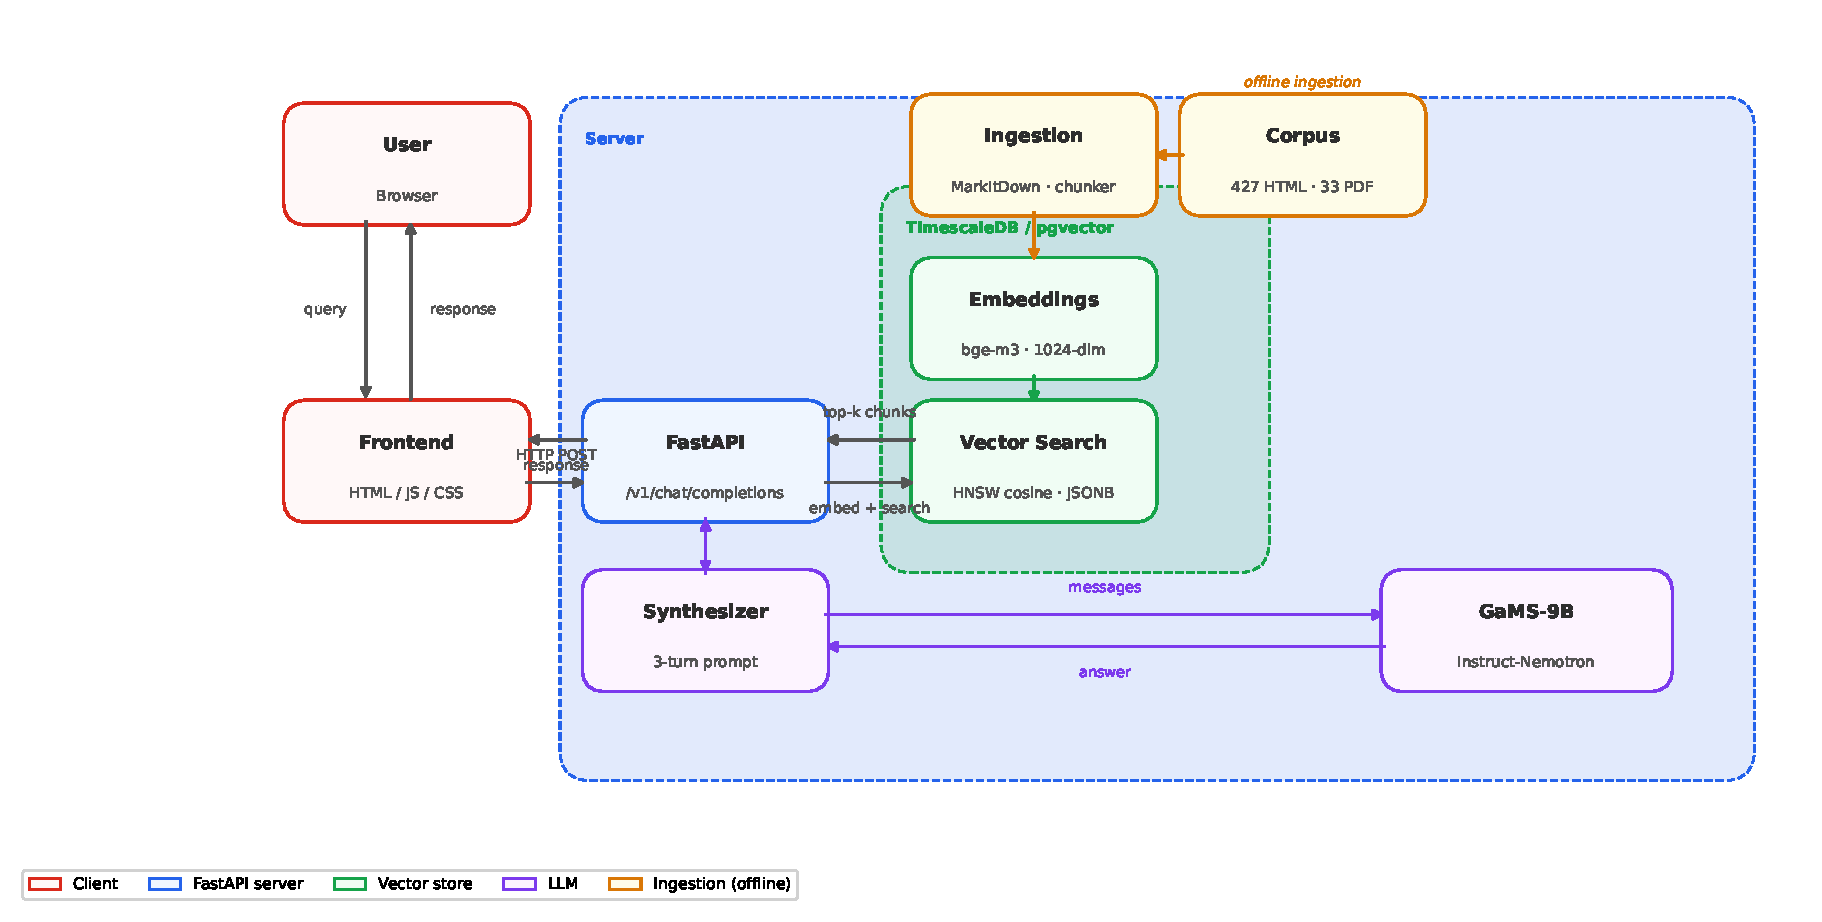
\includegraphics[width=\linewidth]{architecture.pdf}
    \caption{\textbf{ReferatBot deployment architecture.} Dashed borders denote logical groups. Orange nodes are offline; all other nodes run at inference time.}
    \label{fig:architecture}
\end{figure*}



\section*{Results}

The final implementation resulted in a functional web-based conversational assistant.
Figure \ref{fig:ui_landing} shows the initial user interface with suggested questions,
while Figure \ref{fig:ui_chat} demonstrates a successful retrieval and synthesis cycle where the bot correctly answers a query regarding year repetition requirements.

\begin{figure}[H]\centering
    \begin{minipage}{0.48\textwidth}
        \centering
        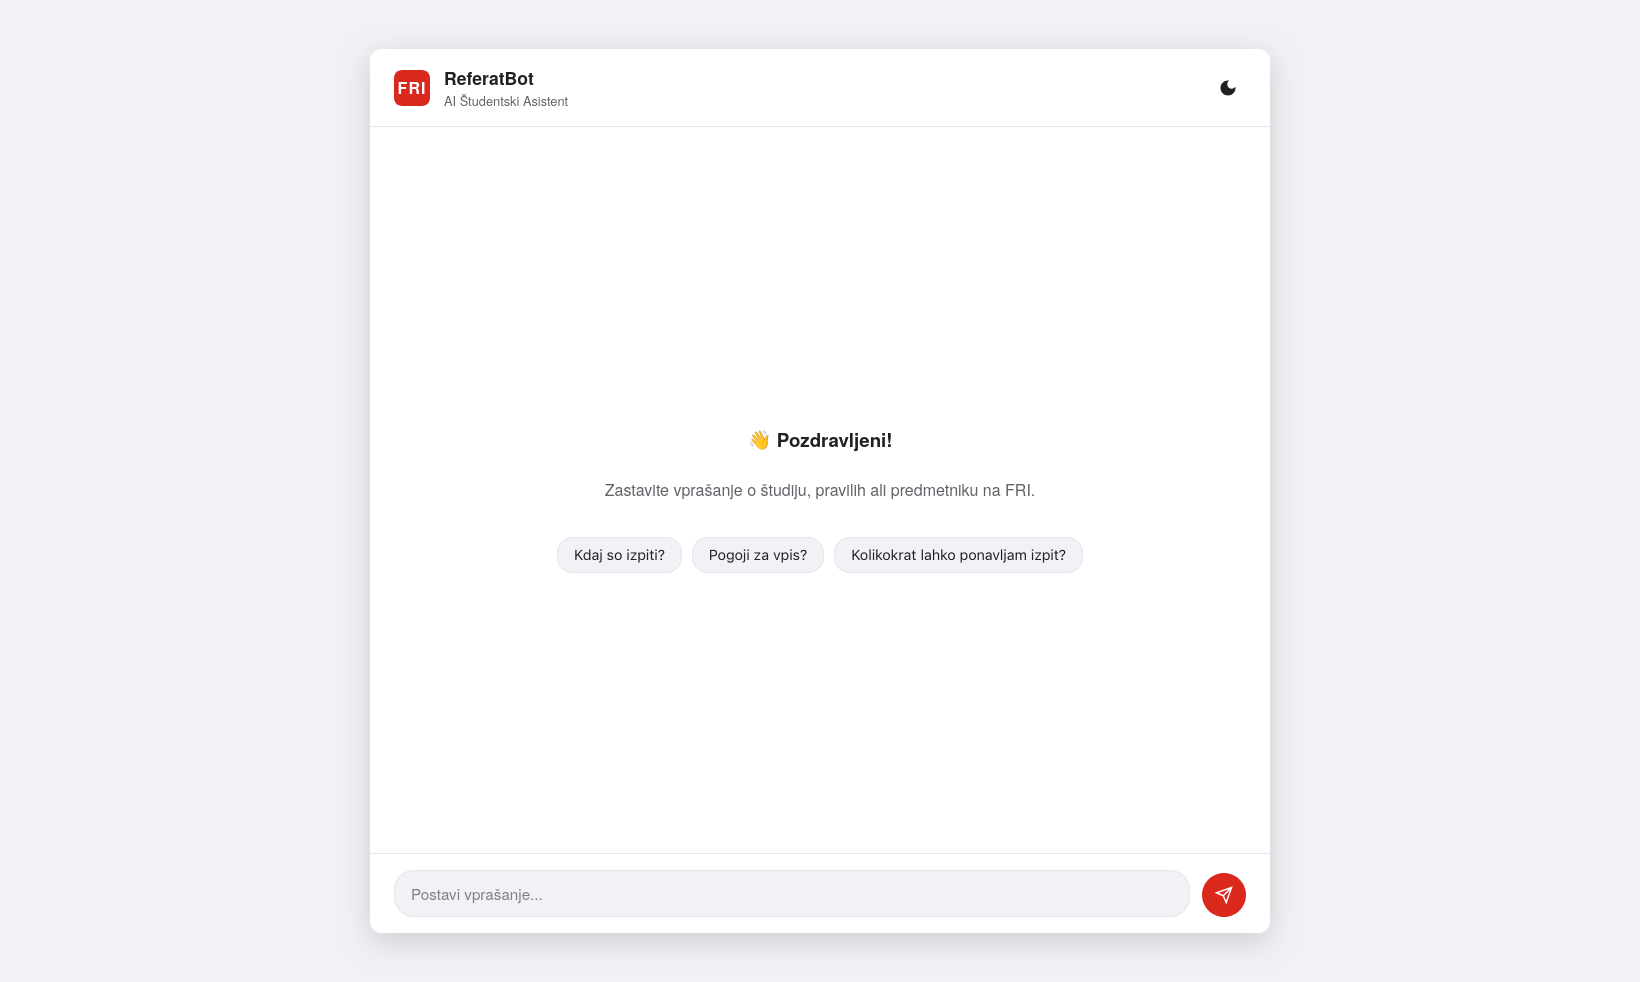
\includegraphics[width=\linewidth]{empty_chat.png}
        \caption{\textbf{ReferatBot Landing Page.} The interface includes a dark mode toggle and suggested starting questions.}
        \label{fig:ui_landing}
    \end{minipage}\hfill
    \begin{minipage}{0.48\textwidth}
        \centering
        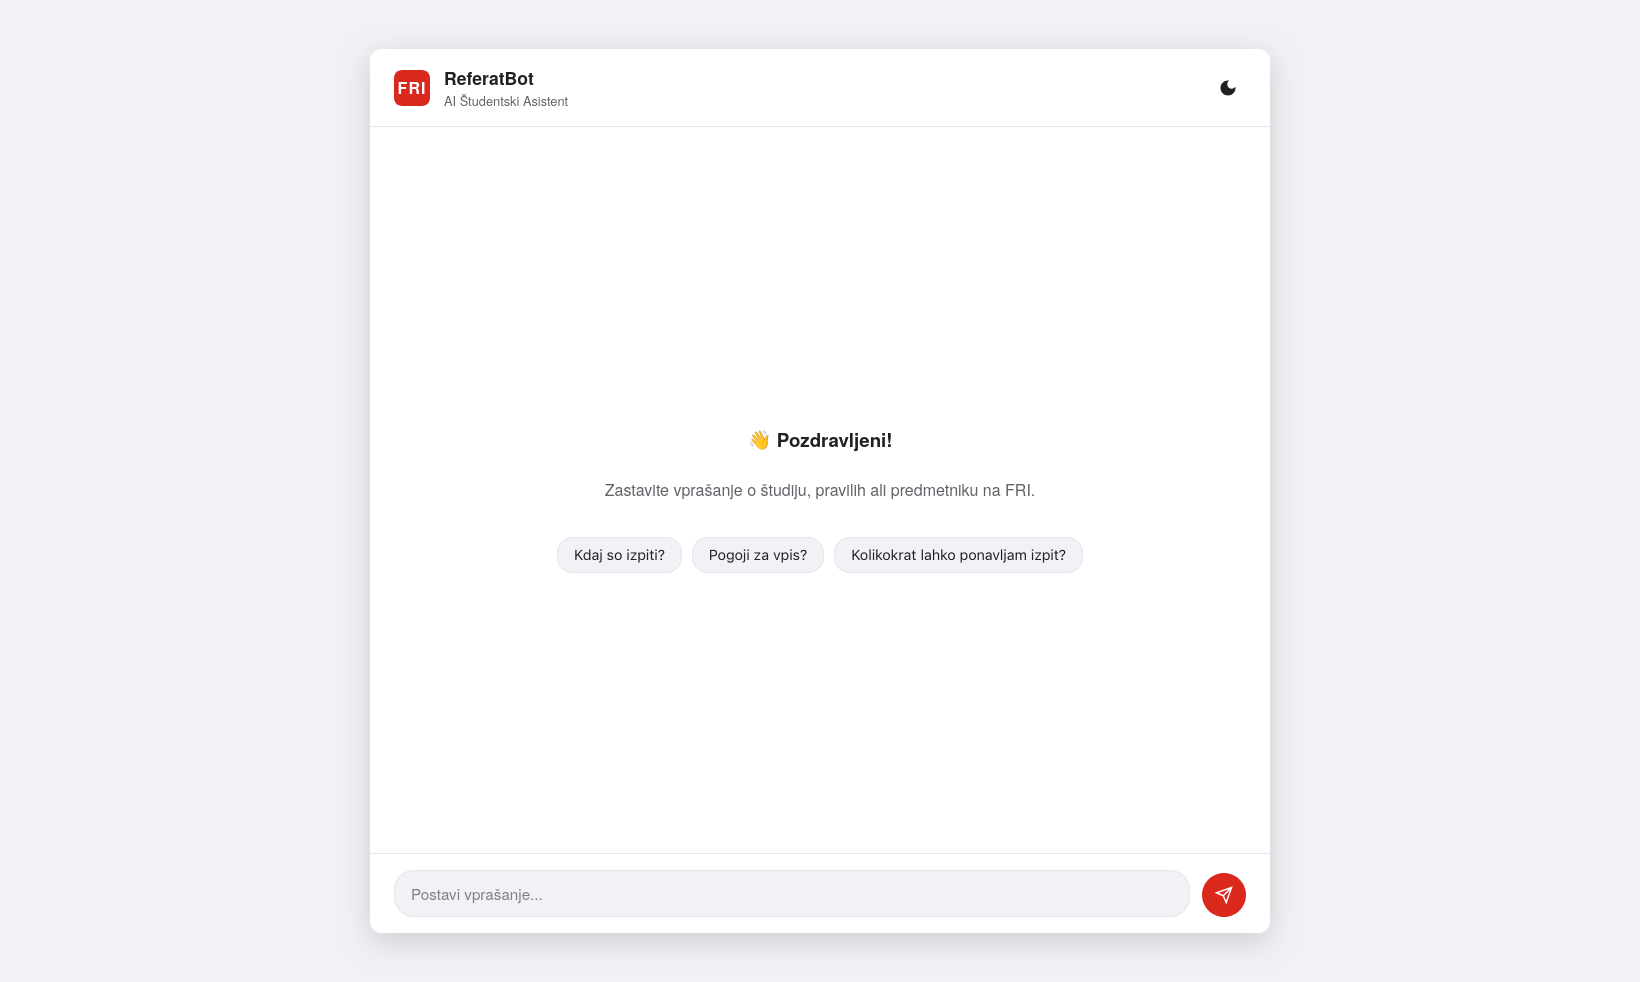
\includegraphics[width=\linewidth]{answered_chat.png}
        \caption{\textbf{Example Conversation.} The bot accurately explains the 30 ECTS requirement for repeating the first year.}
        \label{fig:ui_chat}
    \end{minipage}
\end{figure}

\subsection*{Embedding Model Comparison}

During development we evaluated three embedding models on our handcrafted FAQ dataset,
scored by whether the correct answer appeared in the top retrieved chunks.
Table~\ref{tab:embeddings} summarises the results.

\begin{table}[hbt]
    \caption{Embedding model accuracy on the FAQ evaluation dataset.}
    \centering
    \begin{tabular}{l c c}
        \toprule
        Model & Dim. & Accuracy \\
        \midrule
        intfloat/multilingual-e5-base \cite{mult-e5-base} & 768 & 64\% \\
        google/gemma-embedding-300m \cite{embedding_gemma_2025} & 768 & 77\% \\
        BAAI/bge-m3 \cite{baai3} & 1024 & 77\% \\
        \bottomrule
    \end{tabular}
    \label{tab:embeddings}
\end{table}

Both bge-m3 \cite{baai3} and gemma-embedding-300m \cite{embedding_gemma_2025} outperformed
multilingual-e5-base \cite{mult-e5-base} by 12 percentage.
Despite same accuracy, gemma-embedding-300m requires HuggingFace authentication,
whereas bge-m3 is publicly available without login, simplifying deployment and community testing.
No significant latency difference was observed between the two despite bge-m3's higher
dimensionality (1024 vs.\ 768), so we selected \textbf{BAAI/bge-m3} for the final system.

To support multi-turn dialogues, we also implemented an LLM-driven query-rewriting step prior to vector retrieval. Evaluation showed the system successfully maintained context across multi-turn follow-up questions.

\subsection*{RAG vs. Vanilla LLM Evaluation}

To quantify the RAG pipeline's effectiveness, we evaluated the GaMS-9B model against a standalone "Vanilla" LLM baseline using a dataset of 20 domain-specific student queries. The RAG-enabled model achieved a manual correctness score of 19/20, vastly outperforming the Vanilla LLM's 4.5/20. Qualitative analysis highlighted several Vanilla LLM failure modes that our architecture resolved:

\begin{itemize}
    \item \textbf{System Hallucinations \& Program Confusion:} The Vanilla LLM frequently invented IT systems (e.g., "e-Študent", fake URLs) and fabricated program names (e.g., "informatika in mediji" for IŠRM). The RAG system correctly identified STUDIS and exact degree requirements.
    \item \textbf{Regulatory Inaccuracies:} Without context, the model hallucinated rules, such as a 14-day exam deregistration deadline and a requirement to pass all exams to repeat a year. RAG accurately retrieved the actual 2-day deadline and the 30 ECTS requirement.
    \item \textbf{False Refusals:} For highly specific factual questions (e.g., naming AI thesis mentors or exam costs), the Vanilla LLM triggered out-of-domain refusal guardrails while the RAG system successfully answered these queries.
\end{itemize}

These results confirm that while the base model possesses strong linguistic capabilities, the RAG architecture is essential for grounding responses in factual, institution-specific knowledge.

\section*{Discussion}
Our implementation of ReferatBot demonstrates that a localized RAG pipeline is highly effective for Slovenian academic administration.
However, several areas for improvement remain. The system currently relies on scraped Markdown data; establishing an automated synchronization pipeline with the faculty's official content management system would ensure regulations are strictly up to date. Furthermore, exploring smaller, highly quantized models for the query-rewriting step could further reduce response latency while maintaining conversational context.

%----------------------------------------------------------------------------------------
%	REFERENCE LIST
%----------------------------------------------------------------------------------------
\bibliographystyle{unsrt}
\bibliography{report}

\clearpage

%----------------------------------------------------------------------------------------
%	APPENDICES
%----------------------------------------------------------------------------------------
\appendix

\section*{Appendix A: Embedding Evaluation Dataset}
\label{app:embedding_dataset}

Table \ref{tab:appendix_questions} lists the 11 handcrafted questions used to evaluate the retrieval accuracy of the three embedding models discussed in the Results section. The full dataset used for the RAG vs. Vanilla LLM evaluation, including manual annotations and failure mode logs, is publicly available in the project repository.

\begin{table}[H]
    \caption{Questions used for the embedding model comparison.}
    \centering
    \begin{tabular}{p{0.05\linewidth} p{0.9\linewidth}}
        \toprule
        \textbf{\#} & \textbf{Question} \\
        \midrule
        1 & According to the instructions for the Master's thesis at UL FRI, how many ECTS credits is the thesis worth, and approximately how many hours of work does this represent? \\
        2 & What is the required duration for the oral presentation during a Master's thesis defense at UL FRI? \\
        3 & To complete a doctoral program at UL FRI, what specific requirement must be met regarding scientific publications before submitting the dissertation for evaluation? \\
        4 & What is the minimum number of credits (ECTS) a doctoral student must complete to advance from the first to the second year of study? \\
        5 & Under what condition can a student apply for an extension of their student status due to health reasons according to the enrollment regulations? \\
        6 & What are the guidelines regarding the use of Generative AI (e.g., ChatGPT) in the preparation of a Master's thesis at FRI? \\
        7 & Which of the following is a criterion for a doctoral student to be awarded the 'cum laude' (with honors) distinction upon completion? \\
        8 & What is the purpose of 'Seminar 5' in the doctoral study process at FRI? \\
        9 & For first-cycle (Bachelor's) students, who must be included in the Commission for evaluation and defense? \\
        10 & In the context of language rules for a Master's thesis at FRI, what is required if a student is granted permission to write the thesis in English? \\
        11 & What are the rules regarding the citation of AI tools in academic work at the University of Ljubljana? \\
        \bottomrule
    \end{tabular}
    \label{tab:appendix_questions}
\end{table}

\section*{Appendix B: Conversational Memory Demonstration}
\label{app:memory_transcript}

To demonstrate the effectiveness of the query-rewriting module, the following transcript illustrates a multi-turn conversation. The user frequently omits the primary subject (e.g., "Student Affairs Office", "thesis") in follow-up questions, yet the system successfully maintains the conversational thread and retrieves the correct context.

\begin{description}[style=nextline]
    \item[User:] Kje se nahaja referat?
    \item[ReferatBot:] Študentski referat se nahaja v prostoru R1.03 na Fakulteti za računalništvo in informatiko v Ljubljani...

    \item[User:] Kdaj so odprti?
    \item[ReferatBot:] Študentski referat je odprt od ponedeljka do petka, od 9:00 do 12:00 in od 13:00 do 15:00...

    \item[User:] A jih lahko kontaktiram kadarkoli?
    \item[ReferatBot:] Ne, ne morete jih kontaktirati kadarkoli. Študentski referat je odprt od ponedeljka do petka...

    \item[User:] Koliko časa imam na voljo za izdelavo diplomskega dela?
    \item[ReferatBot:] Na podlagi navedenega konteksta imate na voljo 10 mesecev časa za izdelavo diplomskega dela od dneva prijave v študijskem informacijskem sistemu...

    \item[User:] Kaj pa za magistrsko delo?
    \item[ReferatBot:] Na podlagi navedenega konteksta imate za izdelavo magistrskega dela čas do 30. oktobra...

    \item[User:] Kaj pa če ne naredim do takrat?
    \item[ReferatBot:] Če ne oddate diplomskega dela do določenega roka, imate dve možnosti: Prošnja za podaljšanje roka... ali Ponovna prijava teme...

    \item[User:] A je isto za magisterij?
    \item[ReferatBot:] Da, pravila za magistrsko delo so podobna kot za diplomsko delo. Če ne oddate magistrskega dela do določenega roka, imate dve možnosti...
\end{description}

\end{document}
